\subsection{LM IFU: integral-field spectroscopy}
\label{ssec:overview_ifu}

In general, the workflow is similar to the \ac{LSS} mode,
except the extensive post-processing stage.
The main difference arises from the need to co-add multiple exposures
to achieve the full resolution, since pixel scales are different:
\begin{itemize}
    \item in the along-slice direction, the sampling is sufficient, ie. above the Nyquist rate;
        at $8.2$ mas per pixel;
    \item in the across-slice direction, the sampling is below the Nyquist rate at
        $20.7$ mas per pixel, and dithering/co-adding of multiple exposures is needed.
\end{itemize}

The ratio of these resolutions shows that at least three exposures shifted by one third of the
pixel size are required. The image is then reconstructed on a square pixel grid of
$8.2 \times 8.2 \text{mas}^2$.

The exposures are taken in two perpendicular field rotations,
so that full resolution is obtained naturally in the along-slice direction
and by dithering in the across-slice direction; in the other sequence of three exposures
these directions are essentially swapped.

The association map is shown in Fig.~\ref{Fig:IfuAssomap}.

% Discussion moved to https://github.com/AstarVienna/METIS_DRLD/issues/100
% \TODO{
% We will consider rearranging the recipes to be in line with the
% imaging pipelines. This would entail handling basic reduction and
% background subtraction for of both science and standard exposures in
% common recipes (\CODE{metis_ifu_basic}, \CODE{metis_ifu_background}),
% then having a recipe to analyse the standard observations
% (\CODE{metis_ifu_std_process}). The science exposures are then fully
% calibrated (\CODE{metis_ifu_calibrate}). A full set of exposures would
% then be assembled and restored with a fully sampled PSF in a
% post-processing recipe (\CODE{metis_ifu_combine}).
% }

Two more changes are foreseen in the IFU recipe cascade:
\begin{itemize}
    % https://github.com/AstarVienna/METIS_DRLD/issues/110
    \item Allow telluric standard stars to be used, similarly to the LSS workflow, and

    % https://github.com/AstarVienna/METIS_DRLD/issues/100
    \item Refactor the recipes such that the common processing steps are in a shared recipe, similarly to the imaging workflows.
\end{itemize}


\begin{landscape}
\begin{figure}[ht]
  \centering
  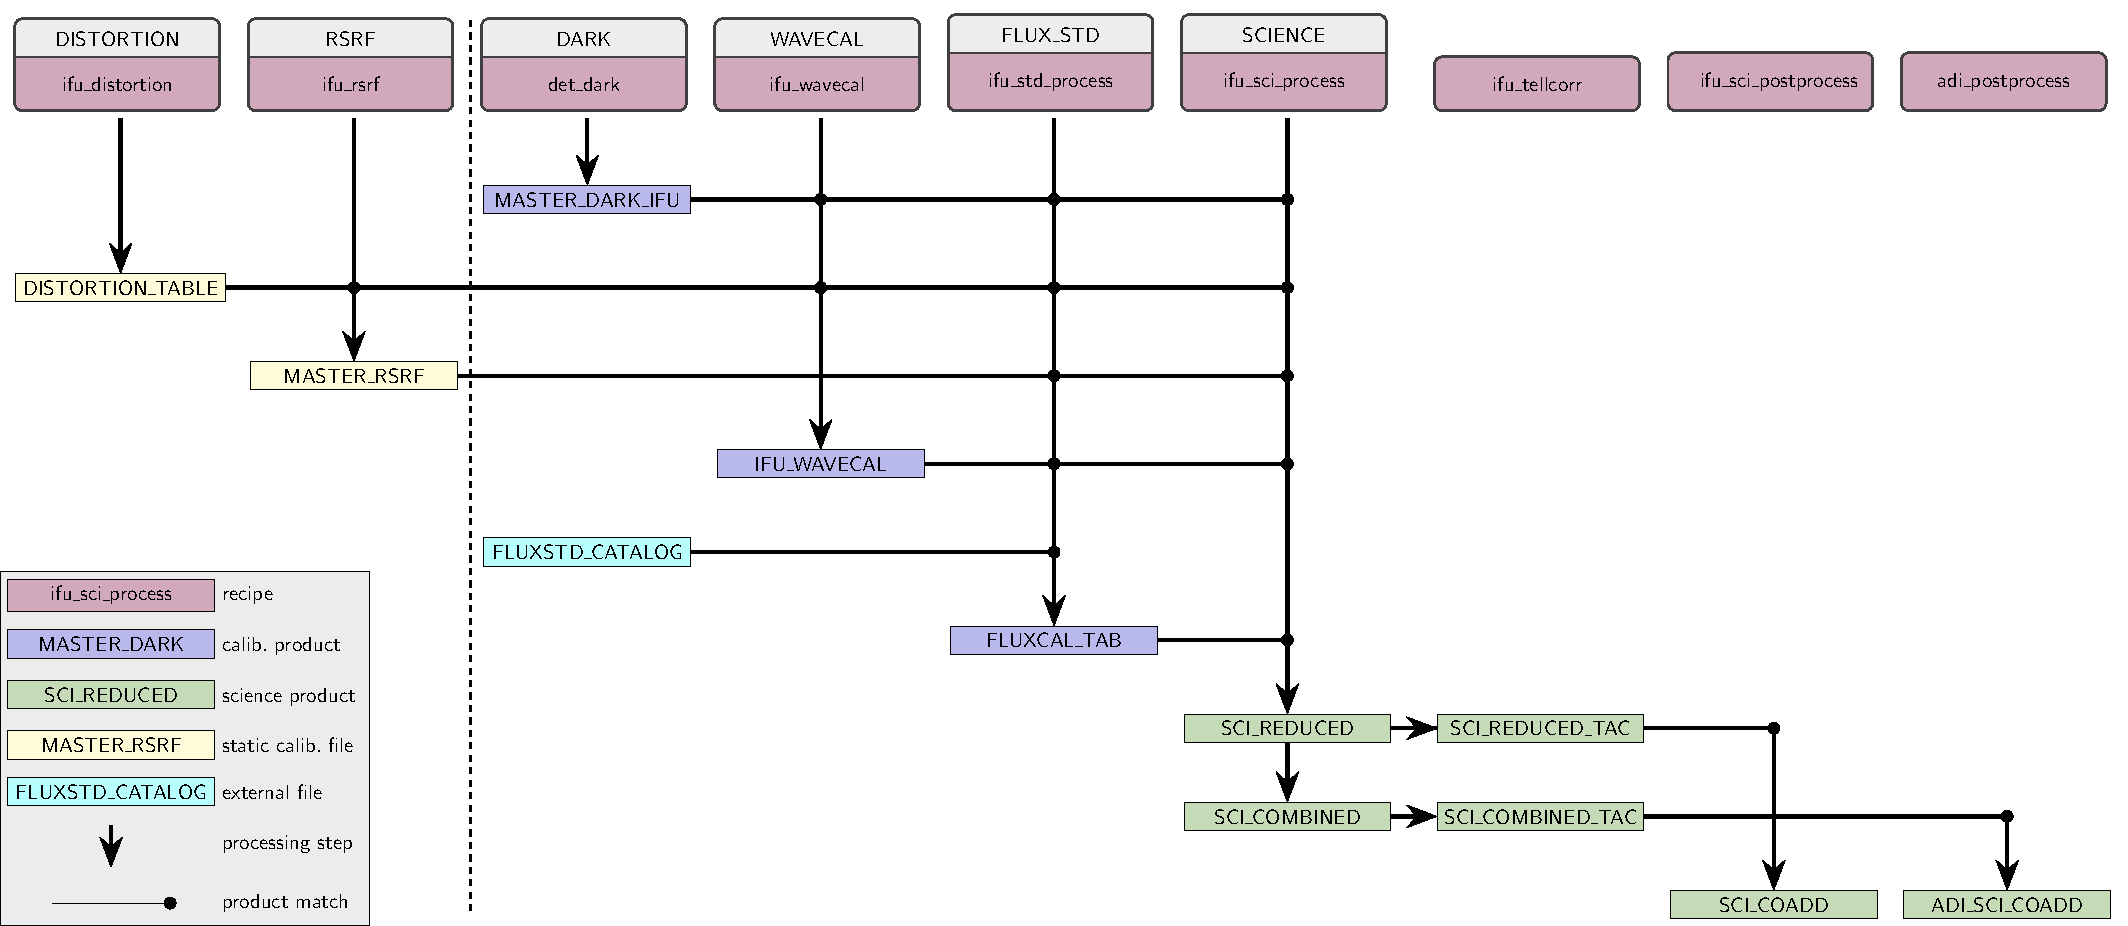
\includegraphics{IFU_assomap_tikz}
  \caption[Reduction cascade and association map for IFU spectroscopy]{%
    Association map for \ac{IFU} spectroscopy in L- and M-band. The
    figure shows only the primary products created by each recipe; for
    a full list of products refer to the recipe descriptions in
    Sect.~\ref{ssec:IFU_recipes}. The dashed line separates
    calibration tasks that are done at AIT or infrequently during
    operations from tasks done daily. The prefix ``\REC{metis_}'' has been
    omitted from the recipe names to improve clarity.}
  \label{Fig:IfuAssomap}
\end{figure}
\end{landscape}



%%%%%%%%%%%%%%%%%%%%%%%%%%%%%%%%%%%%%%%%%%%%%%%%%%%%%%

%%% Local Variables:
%%% TeX-master: "METIS_DRLD"
%%% End:
